\section{Workflow}
\label{sec:workflow}

This section describes what \alibz\ does to one spectrum, in the order in which it does it:
the inputs and outputs of each stage, the gates that decide whether a stage's result is
used, and what each stage was measured to do on real data.
The physics is not repeated; equation numbers refer to Section~\ref{sec:theory}.
Numerical defaults are collected in Appendix~\ref{app:params}, and
Table~\ref{tab:stages} summarizes the stages.
The spectra quoted below are drill-core and mineral spectra from the datasets of
Section~\ref{sec:datasets}; the sample is named wherever a number is attributed to one.

The pipeline runs a blind fit, a provisional identification (pass~1), a physics-conditioned second identification (pass~2) and a deepening stage that re-solves at a frozen plasma state.
Every stage that can change the peak table is either \emph{additive} (it records a diagnostic) or \emph{gated} (it must pass an explicit test against the data), and only the two identification passes may move the plasma state.

\begin{table*}[t]
\centering
\caption{Stages of the \alibz\ workflow. Module names refer to the \texttt{alibz} package;
defaults are listed in Appendix~\ref{app:params}.}
\label{tab:stages}
\footnotesize
\setlength{\tabcolsep}{4pt}
\begin{tabular}{@{}p{0.14\textwidth}p{0.19\textwidth}p{0.27\textwidth}p{0.3\textwidth}@{}}
\toprule
Stage & Module & Input $\to$ output & Gate or decision \\
\midrule
Background & \texttt{peaky\_finder} & raw $y(\lambda)$ $\to$ baseline-subtracted $y$ & per-segment arPLS; fixed physical smoothing length; no smoothing across detector junctions \\
Detection and fit & \texttt{peaky\_finder} & $y$ $\to$ peak table $[A,\lambda_0,\sigma,\gamma]$ & strict local maximum; $\ge 3\sigma$ local noise; width and $2\sigma$-height filters \\
Refinement (3a) & \texttt{refinement} & peak table $\to$ split/merged table & S/A/B models by noise-rescaled BIC; blend needs two distinct database lines \\
Registration & \texttt{wavelength\_\allowbreak{}registration} & peak table, database $\to$ per-segment axis shift & Ar~I/O~I anchors (NIR); $\ge 3$ lines per segment; shift applied only if significant \\
Pass-1 solve & \texttt{peaky\_indexer\_v3} & table $\to$ provisional $(T,\nel)$, composition & detectability $z\ge 3$; stage-consistency tie; collapse guard \\
Refinement (3b) & \texttt{refinement} & deferred asymmetric features $\to$ non-destructive SA tags & resonance-capable lower level; $\tau<\tau_{\max}$; conditioned on retained candidates \\
Seeding and recovery & \texttt{minor\_lines}, \texttt{profiles} & established elements $\to$ added, deblended lines & Boltzmann trust and falsification gates; prior-free area plus BIC \\
Pass-2 solve & \texttt{peaky\_indexer\_v3} & augmented table $\to$ final $(T,\nel)$, composition & as pass~1, warm-started \\
Deepening & \texttt{pipeline} & confident ions $\to$ faint lines, re-solved at fixed state & lowered bar only near own database lines; rejected wholesale on collapse \\
SA recovery & \texttt{profiles} & sa-like peaks $\to$ emission areas, linear re-solve & BIC $\ge 10$; amplification $\le 5$; doublet-anchored species skipped \\
Detections & \texttt{detections} & composition $\to$ status, upper limits, contests & $z\ge 3$ detected; rival cover $\ge 50\%$ $\Rightarrow$ confounded \\
Outputs & \texttt{cli}, \texttt{pipeline} & all of the above $\to$ CSV, JSON, notebook & provenance manifest written unless disabled \\
\bottomrule
\end{tabular}
\end{table*}

Figure~\ref{fig:overview} shows the whole chain applied to one real spectrum, from the raw counts and fitted background to the per-peak residual in units of the local noise.

\begin{figure*}[t]
\centering
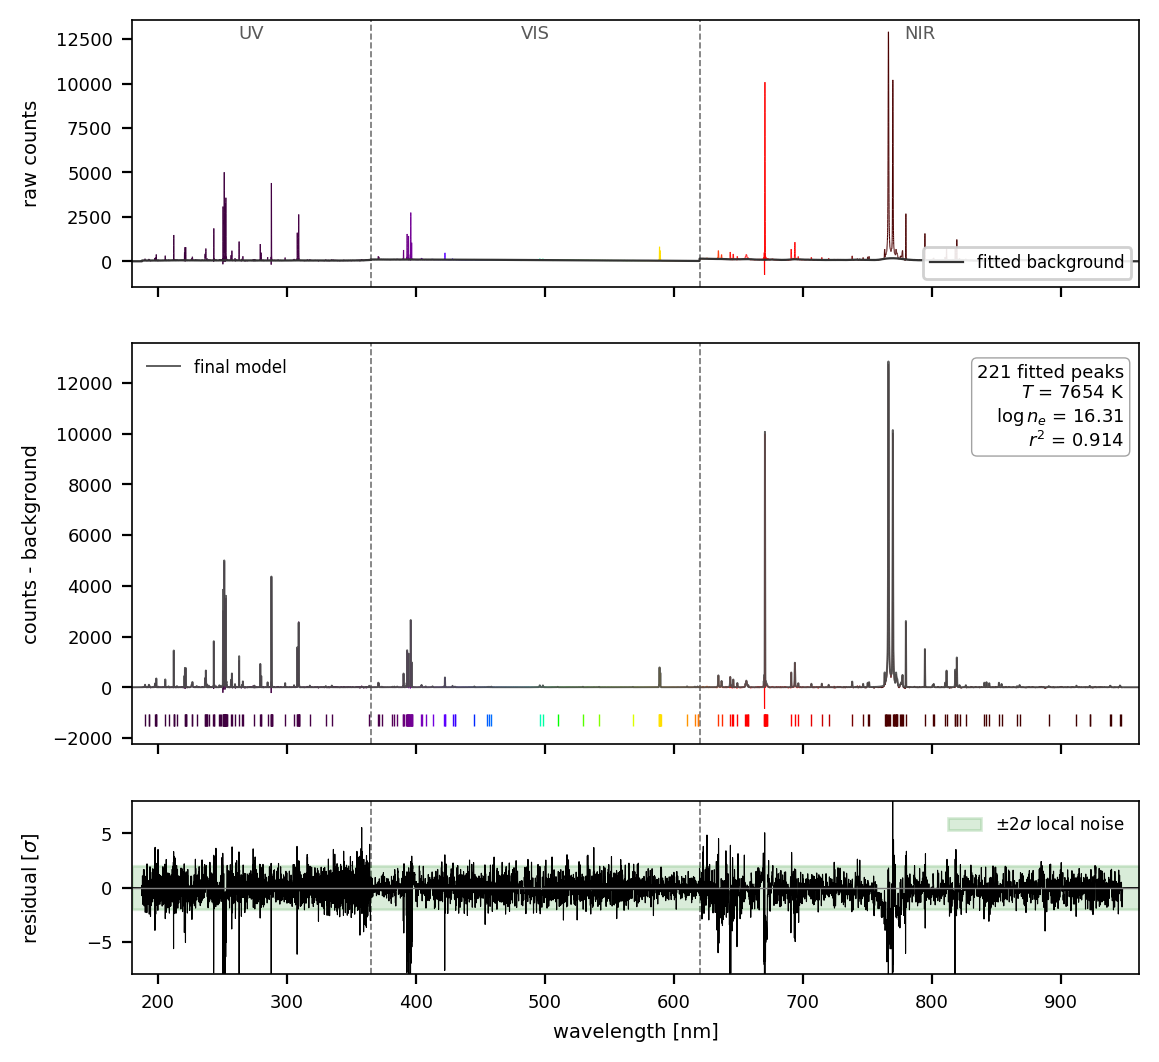
\includegraphics[width=\textwidth]{F1-overview}
\caption{Pipeline overview on the \texttt{user\_spec1} field spectrum. (a)~raw counts with the fitted background; (b)~background-subtracted data with the final model and a wavelength-tinted tick at every fitted peak centre; (c)~residual in units of the local noise $\sigma$ with the $\pm2\sigma$ band. Dashed lines mark the SciAps segment seams at 365 and \SI{620}{\nano\metre} that separate the UV, VIS, and NIR detector segments; the residual structure that exceeds the band is self-absorption, not noise: the largest excursion ($\approx-7\sigma$) is at Li\,I \SI{670.8}{\nano\metre}, with further structure at the Ca\,II H\&K and K\,I 766/\SI{770}{\nano\metre} resonance lines.
The final solve retains 221 fitted peaks and converges to $T=\SI{7654}{\kelvin}$, $\log_{10}(n_e/\mathrm{cm^{-3}})=16.31$, and $r^2=0.914$. % src: manuscript/figures/cache/user_spec1.json
\label{fig:overview}}
\end{figure*}

\subsection{Instrument and data model}
\label{sec:wf-instrument}

The instrument for which the pipeline was developed and validated is a SciAps Z300
handheld LIBS analyzer operated under an argon purge.
Its spectrometer records three CCD segments covering the ultraviolet, visible and
near-infrared, with junctions at \SI{365}{nm} and \SI{620}{nm}.
Each segment has its own wavelength-to-pixel map, so the pixel pitch is not constant:
approximately \SIrange{0.096}{0.079}{nm} per pixel in the ultraviolet segment,
\SIrange{0.142}{0.113}{nm} in the visible, and \SIrange{0.198}{0.156}{nm} in the near
infrared.
A line of a typical width of \SIrange{150}{320}{pm} therefore spans only about
$1.3$--$2.2$ pixels full width at half maximum, at or below the Nyquist limit in the visible
and near infrared.
The junction at \SI{620}{nm} also carries a gain step of roughly a factor of five, which would distort the cross-segment intensity ratios on which Boltzmann and Saha inference relies; it is estimated from the continuum and divided out of amplitudes and uncertainties before every solve (the step at \SI{365}{nm} is additive and is left to background subtraction).

The native record of one acquisition contains 7{,}914 samples.
Of these, 2{,}066 form a fourth, placeholder channel at \SIrange{960}{961}{nm} that carries
no signal and is excluded, leaving 5{,}848 usable samples from \SI{187.8}{nm} to about
\SI{951}{nm}, with a real gap of about \SI{12}{nm} at the red end of the near-infrared
segment that must be masked rather than interpolated.
The vendor's own export resamples the native pixels onto a uniform
\SI{0.0333}{nm} grid with a cubic spline, and an earlier acquisition path used linear
interpolation onto the same grid.
Neither adds information.
In a paired comparison on eight iron runs stored in both forms from the same shots, noise in
the native samples was white (lag-one autocorrelation 0.12), whereas the linearly
interpolated file was strongly correlated (0.76), so a resampled spectrum looks smoother
without being more informative.
\alibz\ therefore processes native pixels.
It accepts any strictly increasing two-column wavelength--intensity file, takes the
pixel pitch from the median grid step, and makes no assumption of a $1/30$~nm grid.
Native fitting required replacing free-width profile fits, which are ill-posed at fewer than
two samples per line width, by estimators that fix the instrument width in pixels
(Sections~\ref{sec:wf-fit} and \ref{sec:wf-registration}).

Two properties of the axis are handled upstream.
Native Z300 spectra initially lacked a pixel offset of $-18$ pixels, so lines appeared \SIrange{1.6}{3.3}{nm} too blue; after the correction a residual of about $-0.25$ pixel remains (Section~\ref{sec:wf-registration}).
The database stores vacuum wavelengths, which the loader converts to the instrument convention (standard air above \SI{200}{nm}, vacuum below) \citep{edlen1966refractive,ciddor1996refractive}; without conversion every line is displaced by \SIrange{0.11}{0.24}{nm}. % src: git 5daafa2 (110-240 pm -> 27 pm median on MW2-112)
Each record analyzed is either a single shot (the MW2-112 scan) or the instrument's own
shot average (ten shots for the Z300 calibration runs); the pipeline treats both as one
spectrum and does not aggregate across records.

\subsection{Background estimation}
\label{sec:wf-background}

The continuum is estimated by asymmetrically reweighted penalized least squares
(arPLS) \citep{baek2015arpls}, a baseline smoother in the family of
Eilers's penalized smoothers \citep{eilers2003smoother}: the baseline minimizes a weighted squared residual plus a
second-difference roughness penalty, and the weight of any pixel above the current
baseline is driven toward zero over successive iterations, so that emission lines of any
width cannot attract the baseline.
Two choices adapt the method to this instrument.
First, the smoothing penalty is set from a \emph{physical} length rather than a number of
pixels: the penalty weight is $(\ell/\Delta\lambda)^4$ for a smoothing length $\ell$ of
\SI{1.9}{nm} and the local pitch $\Delta\lambda$, so the stiffness is the same on all three
segments and on any wavelength grid.
Second, the spectrum is split at the detector junctions and each segment is solved
independently, so that the penalty never spans a hardware step.
On MW2-112 the omission of this split left a $+54$-count ledge at \SI{620}{nm} that
produced spurious peaks; with per-segment solves the ledge was removed.

A failed baseline solve falls back to a zero baseline, and segments are not blended across junctions, so a line straddling \SI{365}{nm} or \SI{620}{nm} is divided between two solves.

\subsection{Peak detection and profile fitting}
\label{sec:wf-fit}

\paragraph{Detection.}
Candidate peaks are strict local maxima: a sample must exceed four of its five window
neighbors.
A maximum is retained only if its intensity exceeds a significance floor of three times
the local noise, and a user-supplied excess is added to, not subtracted from, that floor.
The local noise is a robust point-to-point estimate (the median absolute successive
difference, scaled to a Gaussian standard deviation, evaluated at several lags and taken at
the largest), computed in blocks that restart at each detector junction so that noise from
one segment does not leak into another.
Flat-topped maxima fail the strict test and are recovered by refinement.

\paragraph{Windowed Voigt fits.}
Each detected peak defines a half-maximum window, within which the line is fitted by a
Voigt profile \citep{olivero1977voigt,thompson1987voigt} with parameters
$[A,\lambda_0,\sigma,\gamma]$, where $A$ is the \emph{integrated area}.
This convention is central: the profile is unit-area normalized, so seeding from a
measured height rather than from an area would overestimate the area of narrow lines by
roughly a factor of four.
The fit is bounded: non-negative area, widths limited to a multiple of the median width, center within one sample of its seed.
The modeled contribution of other fitted peaks is subtracted from each window first, so that strong wings do not act as an unmodeled pedestal.

\paragraph{Shoulders and block-coordinate refit.}
Residual structure above two standard deviations of the residual is searched for
unmodeled maxima, and a new component is added wherever one lies farther than one
linewidth from an existing peak, with the existing peaks held fixed.
The components are then refitted jointly, strongest first, in overlapping blocks of
$\pm 50$ samples, the out-of-block components being subtracted as a fixed pedestal.
This is a block-coordinate refit, not a single joint solve over several hundred peaks.
The widths are capped at the window span.
The cap was added after an unbounded fit allowed a single component of
$\sigma = \SI{289}{nm}$ to absorb \SI{89}{\percent} of the fitted area of its window.
Finally, components wider than one hundred times a robust median width
(baseline remnants) are discarded, sub-sample widths are set to zero, and a component
survives only if its implied height exceeds twice the local noise.
On MW2-112 spectrum~0, this first pass returned 303 peaks.

\paragraph{Per-segment peak location.}
Because the lines are barely sampled (Section~\ref{sec:wf-instrument}), the way a line
center is read from the samples matters at the picometer level.
A paired study on 26 iron and 87 vanadium runs on the corrected axis compared a
three-point parabola, a root of the vendor-style cubic spline, a free-width pixel-integrated
Gaussian, and an empirical line-spread function (ePSF) built from the data
\citep{anderson2000epsf}.
No single estimator was best on all segments.
In the visible, the ePSF located iron lines with an error of \SI{5.3}{pm}, against
\SIrange{11.6}{12.3}{pm} for the spline-based estimators.
In the ultraviolet the spline estimators were better (\SIrange{4.7}{4.8}{pm} against \SI{7.6}{pm}), and in the near infrared, tested on argon~I lines because iron lines are absent, a point Gaussian beat the spline (\SI{4.8}{pm} against \SIrange{14}{15}{pm} at \SI{696.54}{nm}); the near-infrared ePSF is withheld because of a location bias at its sub-band seams.
The pipeline therefore dispatches the location method \emph{per segment}, from a packaged
shape file (ePSF in the visible, spline root in the ultraviolet, point Gaussian in the
near infrared), and falls back to the spline root or the Gaussian refinement for any grid
that is not recognized as Z300-native.
The located centers and fit diagnostics are recorded for every refined peak and drive the wavelength registration; the identification stages still consume the blind Voigt centers, pending a dedicated accuracy benchmark.

\subsection{Refinement: blends, phantoms and self-absorption tags}
\label{sec:wf-refinement}

A first-pass fit with symmetric profiles fails in two ways on real spectra.
A self-absorbed, flat-topped line is split into two \emph{phantom} components, and a
genuine blend narrower than one linewidth is fitted as one component.
The refinement stage re-examines every ambiguous feature (sub-linewidth pairs of
components and significant residual structure) under three local models: a single
symmetric Voigt (S), a Voigt attenuated by a cold absorber of the same shape, the
self-absorption profile of Eq.~\eqref{eq:sa-voigt} (A), and two symmetric Voigts (B).
The models are compared by the Bayesian information criterion \citep{schwarz1978bic},
with the raw $\chi^2$ rescaled by the reduced $\chi^2$ of the best model (floored at one),
so that the margin measures relative improvement on windows dominated by systematic
residuals rather than by photon noise.
Fits use a robust soft-$L_1$ loss \citep[cf.][]{huber1964robust} whose scale leaves the five-to-seven-sigma Voigt misfit on the brightest lines un-downweighted, since that misfit is model inadequacy and not outlier contamination.

The verdict is then gated by physics.
A blend is accepted only if the database supplies two \emph{distinct} lines matching the
two fitted centers with a consistent separation, with a BIC margin of 10 (30 without
database support).
An asymmetric verdict is applied only if the primary line has a resonance-capable lower
level ($E_i \le \SI{0.2}{eV}$), the class of lines that self-absorb, and the fitted
emission center has not walked off that line; otherwise it is recorded under a qualified
verdict (nonresonant, displaced or saturated) and left alone.
A fitted optical depth at the fit ceiling is never acted on.

Refinement is staged.
Stage~3a runs before any identification and applies only the data-only actions (blend
splits and single merges), deferring the whole asymmetric family.
Stage~3b runs after pass~1, when a provisional element posterior exists, and adjudicates the
deferred features with the resonance gate conditioned on the \emph{candidate species the
whole-pattern solve retained}, a set broader than the established elements (so that a
wrong pass-1 basin cannot veto a real resonance merge) but far narrower than the periodic
table.
The merge zones are computed before any seeding, and the seeder, residual recovery, deblending and self-absorption recovery all honor them; seeds that landed inside merge zones had eroded the observed areas of merged rows by \SIrange{21}{93}{\percent}.

A merged self-absorbed row carries two areas, and the distinction is important for
quantification.
The \emph{observed area} is the integral of the attenuated profile actually seen, corrected
for the Lorentzian flux outside the fit window.
The \emph{emission area} is the unattenuated, thin-equivalent area of Eq.~\eqref{eq:escape},
proportional to the quantity that enters Eq.~\eqref{eq:emissivity}.
The first version of the merge replaced the fitted components by the narrow absorbed core of the self-absorption model with its wing-inflated area; on MW2-112 spectrum~1000 this overshot the observed core by up to $19\sigma$ at \SI{280.2}{nm}, deleted neighbors that reappeared as $40\sigma$ residuals, and almost doubled the global $\chi^2/\sigma^2$ (32{,}821 after stage~3a to 51{,}701 after 3b).
The verdict is therefore now a \emph{non-destructive tag}: the table keeps the data-faithful symmetric fit, and the emission area and optical depth ride along as metadata for the later growth-curve recovery.
With tags, stage~3b improves the fit (to 28{,}262) and unmodeled residuals above $3\sigma$ fall from 61 to 28.
The symmetric proxy conserves flux but not shape and therefore leaves a core-shaped residual on a flat-topped line, which is a storage choice and not a failure of the model.
On MW2-112 spectrum~0 the residual of the self-absorption model in each merged window was
2--8 times lower than that of the stored symmetric proxy (Li~I \SI{670.7}{nm}, K~I
\SI{766.5}{nm}, Fe at \SI{261.2}{nm}), and the ratio of emission to observed area ranged from 1.24
to 7.0 over fifteen merged lines.
The one genuine cost occurs in crowded windows: where seven components collapse into one (\SI{383.0}{nm}) the model underfits (residual 549 against 76 for the two-phantom fit).
The refinement reduced the first-pass fit from 303 to 288 peaks.

Two further profile-level actions run after the identification passes, each gated and
excluded from merge zones.
\emph{Shoulder deblending} refits a peak whose residual shows a one-sided flank bump as two
components plus a pedestal, the main component confined near its parameters and the new
one pinned at the bump, accepted at a matched-filter signal-to-noise ratio of 4 and a window
BIC margin of 6.
\emph{Self-absorption area recovery} (Section~\ref{sec:wf-solve}) refits sa-like peaks
of species that are not already doublet-anchored.
On the 38 JChristensen drill-core spectra, deblends fired on 26 and recovery on 24.
Figure~\ref{fig:refinement} shows the two resonance-line decisions on MW2-112 spectrum~1000.

\begin{figure*}[t]
\centering
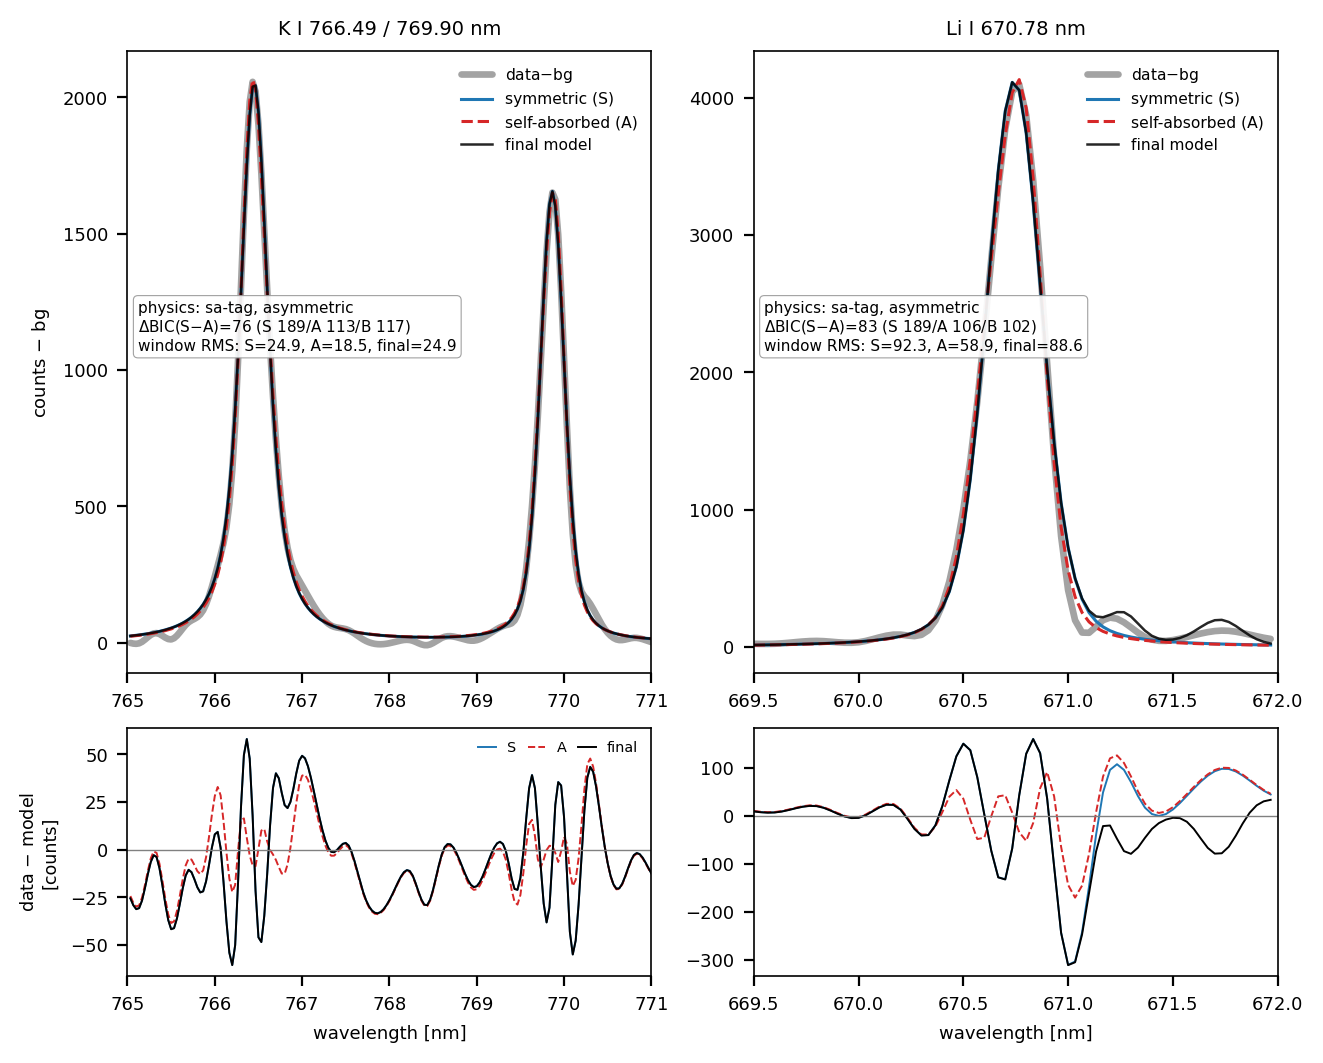
\includegraphics[width=\textwidth]{F3-refinement}
\caption{Self-absorption refinement in two resonance windows of MW2-112 spectrum~1000 (the K window spans both the 766.49 and \SI{769.90}{\nano\metre} doublet lines): the symmetric single Voigt (S), the self-absorbed profile of Eq.~\eqref{eq:sa-voigt} (A), the final model, and the three residuals below. On this spectrum both lines are resolved as non-destructive self-absorption \emph{tags} (verdict asymmetric), not as the phantom-split merge seen on spectrum~0: the tag keeps the data-faithful symmetric envelope in the model (so the final residual tracks S) while recording the attenuated-emission metadata, and the A profile that fits the reversed core more closely is the statistically preferred shape.
K\,I \SI{766.49}{\nano\metre} gives $\Delta\mathrm{BIC}(S{-}A)=76$ with in-window residual RMS of 24.9 (S), 18.5 (A), and 24.9 counts (final); Li\,I \SI{670.78}{\nano\metre} gives $\Delta\mathrm{BIC}=83$ and RMS 92.3, 58.9, and 88.6. % src: manuscript/figures/cache/mw2_1000.json
\label{fig:refinement}}
\end{figure*}

\subsection{Wavelength registration}
\label{sec:wf-registration}

Matching a peak table against a database requires an axis registered to a few tens of picometers, so registration is measured on each spectrum.
The most trusted references are the Ar~I and O~I lines that are present because of the
argon purge and the ambient air; they are independent of the sample and lie almost
entirely in the near-infrared segment.
Their set of anchors (696.5, 706.7, 738.4, 750.4, 763.5, 772.4, 794.8, 801.5, 811.5, 826.5,
842.5 and \SI{912.3}{nm}) registers as genuine argon to within about $\pm\SI{30}{pm}$ on
the corrected axis, with ten to twelve clean lines per run, so that the near-infrared segment
passes its three-line gate on essentially all runs.
Second, a deterministic estimator measures \emph{golden lines} of the declared composition,
selected as lines in the segment's strongest predicted set with no composition, argon,
nitrogen, oxygen or hydrogen line of non-negligible strength within $\pm\SI{0.5}{nm}$,
centered by the point-Gaussian fit and combined by a Huber estimate into a per-segment
offset; fewer than three golden lines leave the segment unregistered.
A vote-mode estimator is retained as a diagnostic only. Only the \emph{offset} is applied; the fitted slope is a diagnostic, because the strongest near-infrared metal lines are optically thick and displaced.

The measured behavior justifies this restraint.
On the corrected axis the residual calibration error is about $-0.25$ pixel in the
near-infrared segment (median $-0.25$ pixel from an Ar~I cross-correlation recorded with each run, $-0.26$ pixel
from the ambient Ar~I shift, 107 runs), but it is \emph{not} a constant: it is $\approx 0$
for one calibration epoch, $\approx -0.28$ pixel for another, and swings from $-0.5$ to $+0.25$
pixel from run to run.
It is therefore a per-calibration residual to be measured on each spectrum, not a fixed
offset.
The per-segment offset transfers between metals (iron to vanadium in the visible: \SI{40}{pm} against \SI{597}{pm} on the uncorrected axis), with a run-to-run standard deviation of at most \SI{12}{pm} in the visible.

The default mode applies the composition-independent ambient registration to the near-infrared segment and keeps the legacy mixed-element anchor shift elsewhere. The element registration is recorded but not applied by default, because changing the inversion's wavelength input pipeline-wide should be gated on an accuracy benchmark.
A second argon-based engine (regional Ar~I and O~I offsets, applied only inside its bracketed anchor support when at least three consistent groups agree) runs alongside; the two argon estimates are cross-checked and a flag is raised beyond three standard errors.
All shifts follow the convention observed $-$ database.

The mixed-element legacy shift is also estimated \emph{per segment}, from the
\emph{refined} table, and a segment's own median is adopted only when it
has at least five unambiguous matches and deviates from the pooled global median by more
than twice the median's standard error.
The gate is essential.
On MW2-112 the per-segment medians differed by \SIrange{10}{35}{pm} but with
median absolute deviations of \SIrange{26}{71}{pm}, so the gate refused and behavior reduced to
the global shift; when the gate was removed, a $+\SI{20}{pm}$ pseudo-shift in one segment
conjured \SI{25}{\percent} phantom Ti in MW2-112 spectrum~1000.

\subsection{Prior-driven minor-line seeding and iterative deepening}
\label{sec:wf-seeding}

Once an element is established from its strong lines, the remaining lines of that element
in the same ion stage are predicted: within one stage, Eq.~\eqref{eq:emissivity} fixes all
line ratios up to a single per-(element, stage) scale, which is measured from the
stage's clean strong lines.
The seeding stage uses those predictions to fit lines the blind pass rejected, and to
deblend an established line hidden beneath a stronger line of another element.
Scale calibration admits a database line as a reference only if its same-element multiplet
contamination is at most \SI{10}{\percent}, its nearest fitted peak lies within \SI{0.06}{nm} and
clears a noise-derived amplitude, and no other peak blends it; the scale is the robust
median of area over predicted strength, and its spread is the median absolute deviation.
A stage predicts only when at least three consistent references exist and the spread is
bounded.
A stage is \emph{falsified} if its brightest predicted line would far exceed anything matched
(the case of a spurious Na~II), and every addition must agree with its Boltzmann prediction
to within a factor of five, or it is recorded as inconsistent or missing and not added.
Importantly, the acceptance decision is made on a prior-\emph{free} area, a non-negative
least-squares area against a frozen-geometry basis \citep{lawson1995nnls}, together with a
BIC improvement: the prior justifies looking for a line, but the data decide whether it is
there.
The module assumes a single reference temperature of \SI{0.76}{eV} ($\approx\SI{8.8}{kK}$,
the corpus median for MW2-112) and optically thin emission, and does not couple ion stages
(the Saha coupling of Eq.~\eqref{eq:saha} belongs to the solve).
On MW2-112 spectrum~0 the first-pass fit of 303 peaks became 288 after refinement and 299
after seeding.

Seeding as a single pass was replaced by \emph{iterative deepening}.
The earlier design seeded once and then re-optimized the plasma state (pass~3), which on drill-core data drifted into a low-temperature basin ($\approx\SI{5200}{K}$) where one line-rich element explained everything while $r^2$ improved.
In the current design, the ions that are \emph{quantified from their intense peaks}, those
with at least four clean reference lines in some stage, have earned a lower
recovery bar for their own faint lines.
In each round, at a successively lower local-noise bar (currently $3.0\sigma$ and then $2.0\sigma$),
these ions are seeded from the Boltzmann prior and, in addition, residual peaks are
recovered from the data without a prior, but only where a confident ion's own database line
marks the position; empty regions keep the full $4\sigma$ bar and cannot admit chance
coincidences.
The composition is re-solved at the \emph{fixed} pass-2 plasma state, so that the weak lines
corroborate and cannot move the temperature; the re-solve reproduced the optimizer's final
solve to machine precision on its own state, and a round is rejected wholesale if it newly
collapses the composition (Section~\ref{sec:wf-solve}).
On MW2-112 spectrum~1000, deepening added 41 lines (23 seeded and 18 recovered) in three
rounds, under an earlier three-bar schedule, without collapse, in about \SI{264}{s} end to end.

\subsection{Whole-pattern solve}
\label{sec:wf-solve}

\paragraph{Candidates and design matrix.}
The solver is run twice, as pass~1 (provisional) and pass~2 (warm-started at the pass-1
state).
For a trial plasma state, every database line of every candidate element and ion stage
contributes a column of the Saha--Boltzmann design matrix (Eqs.~\eqref{eq:emissivity} and
\eqref{eq:saha}), and the observed peak areas are modeled as the non-negative combination
of columns that minimizes the amplitude misfit.
Candidates are pruned by an evidence prefilter, and a provisional pass-1 rejection cannot
prohibit later recovery, because passes~2 and deepening rebuild their candidates from their
own peaks.
The default objective is the non-negative least-squares fit; the weighted variant
(Eqs.~\eqref{eq:wnnls} and \eqref{eq:sigma-eff}) is implemented but is an opt-in, since in
tests on synthetic Ca--Mg scenes it was accurate at the true plasma state but its $\chi^2$
still misranked the temperature; it stays off until that bias is resolved on the synthetic suite.
When the weighted solve is used, the additive amplitude floor of Eq.~\eqref{eq:sigma-eff} is
set from the spectrum's own noise scale, because the sigma from the fit collapses where
the local window is quiet.

\paragraph{Plasma state.}
Temperature and electron density are found by a search over $(T,\log_{10}\nel)$.
The default search evaluates a $15\times 7$ grid of profile objectives and seeds a
Gaussian-process optimizer \citep{jones1998ego} from it; the grid became the default because
the objective has a narrow valley along the Saha $(T,\nel)$ ridge, which the
cold-started optimizer missed on every spectrum tested, and the grid seeds land on the ridge.
The amplitude objective is flat in $\nel$ at fixed temperature, so $\nel$ is set by a prior:
the Stark width of H$_\alpha$ \citep{gigosos2003halpha} when present, and otherwise a default of
$\log_{10}\nel = 17.0 \pm 0.5$ (in cm$^{-3}$) with the search restricted to
$\pm 1\sigma$ of it.
The restriction costs no data fidelity, since the objective is flat in $\nel$, and
it prevents the stage-consistency thermometer, which sees $\nel$ only through the Saha
degeneracy, from sliding to the cold end of the ridge.
In the synthetic Ca--Mg tests this box gave Ca/Mg $=0.52/0.48$ at \SI{8.9}{kK} (truth $0.6/0.4$ at
\SI{10}{kK}), whereas a $2\sigma$ box gave \SI{8.2}{kK} and a wrong order.
A result at the edge of the box is flagged.
The cost includes the stage-consistency term of Eq.~\eqref{eq:tie-cost}, weighted at unity,
so that the Saha--Boltzmann stage ratio is trusted exactly as much as the observed amplitudes;
setting the weight to zero recovers the historical thermometer based on within-stage
Boltzmann ratios only.

\paragraph{Collapse guard.}
On drill-core spectra the single-element dominance failures (Hg at 1.000, Fe at 0.991,
Ca at 0.990) were \emph{not} peak-shape failures: the driver peaks classified as
instrumental.
They were inverse-solve basin failures, in which a corroboration re-index drifted to a
low-temperature basin where one element's tiny response explained everything while
$r^2$ \emph{improved} (to 0.87), because a line-rich element can fit anything.
A corroborated composition is therefore rejected when its top fraction reaches
\SI{90}{\percent} and has grown by at least $0.2$ over the pass-2 top fraction; the summary records
\texttt{corroboration-rejected(collapse)}.
In A/B tests Hg 1.000 became K, Li and Si, and Fe 0.991 became Si, K and Li.
The guard complements shape quality control, which flags abundances resting on saturated or overlap-contaminated peaks; goodness of fit alone cannot compare basins.

\paragraph{Detectability gate.}
An element is dropped if its strongest predicted line does not clear $z_{\min}=3$ times the
local \emph{area} noise of the peak, a statistic (Eq.~\eqref{eq:detect}) that is immune to a
single dominant line and admits arbitrarily many low-concentration elements provided each
shows one real line above noise.
Without a noise model (a bare indexer) only a zero-column activity test applies, so the gate
cannot over-exclude in code paths lacking one.
On MW2-112 spectrum~1000, Bi, which pass~1 had assigned a fraction of 0.94 on the strength of an
ill-conditioned estimate whose predicted strongest line was four counts, had $z = 2.2$,
against $z \ge 4.6$ for every real element (Mn 4.6, Be 6.8, up to K at 103); the gate also
removed an Hg phantom (0.27, $z=0.5$) and left a silicate assemblage of Si 0.75, Fe 0.09,
Al 0.05 and Ti 0.04 together with the real Be, Rb, Na and Ca traces.

\paragraph{Confounder contest and resolution.}
For every detected element, the contest of Eq.~\eqref{eq:contest} asks whether a rival could
cover the element's supporting peaks without violating its own true negatives, scanning a
corpus-plausible plasma grid ($T\in\{6,8,10,12\}$~kK, $\log_{10}\nel\in\{16.5,17.5\}$)
against a pre-prune candidate table built at \SI{9}{kK}, because a wrong attribution drags
the fitted state to where the rival's lines vanish and the error then certifies itself.
A supporting peak is contested if a rival, at the largest concentration its own true
negatives allow, still covers at least half of the peak's amplitude, using the rival's
non-resonance lines to set that cap so that self-absorbed resonance lines do not
understate it.
An element whose every supporting peak is contested is demoted to \emph{confounded}.
On the drill-core spectra, two hot-Mn results (40--53\,\% Mn, resting on two peaks inside
the Mg~II 279.553/\SI{280.270}{nm} doublet region) were demoted with a contested share of 1.0
and the confounder Mg, while independent Li, Al and Na detections were untouched.
The reported composition then credits a confounded element only its clear flux and
reattributes the contested remainder to the confounder, under two guards: the response
ratio is clamped at one, and a rival receives flux only up to its own evidence ceiling
(zero if the fit pruned it).
Without the first guard a 3.8\,\% Be confound became a 42\,\% Fe phantom.
The result is Mn $53\%\to 0\%$ and Mg $8\%\to 31\%$.

\paragraph{Self-absorption recovery re-solve.}
For sa-like peaks of species not anchored by a resolved doublet, the self-absorption model
is refit against a symmetric control, accepted only with a BIC win of 10, an optical depth
below the ceiling, and an amplification of at most five.
Accepted emission areas replace the observed amplitudes, and the composition is
\emph{re-solved linearly} at the fitted plasma state, with no new Bayesian pass and no basin
risk, and the collapse guard is applied to the corrected composition as a final safeguard.
Doublet-anchored species (K~I, Na~D) are skipped, since their depths already act on the response side and correcting the data side too would double-count.
The pre-measured emission-to-observed ratios of merged lines are propagated through the same re-solve.
On the JChristensen set, corpus means moved by $+3.1$ percentage points (Si) and $-3.5$ (K) with no collapse; on MW2-112 the recovered lines (Al~I \SI{396.1}{nm}, Mg~I \SI{383.8}{nm}) carried optical depths near $0.5$.

\paragraph{Uncertainties.}
Statistical uncertainties on the fractions come from resampling the peak amplitudes within
their uncertainties (32 draws by default) and re-solving at the fitted state
\citep[cf.][]{efron1979bootstrap}.
They do not include the systematic error of the LTE assumption, of the atomic data, of matrix
effects or of unresolved self-absorption, and the reported fractions should be read
accordingly.

Figure~\ref{fig:walkthrough} follows MW2-112 spectrum~1000 through the stages and across the successive solves.

\begin{figure*}[t]
\centering
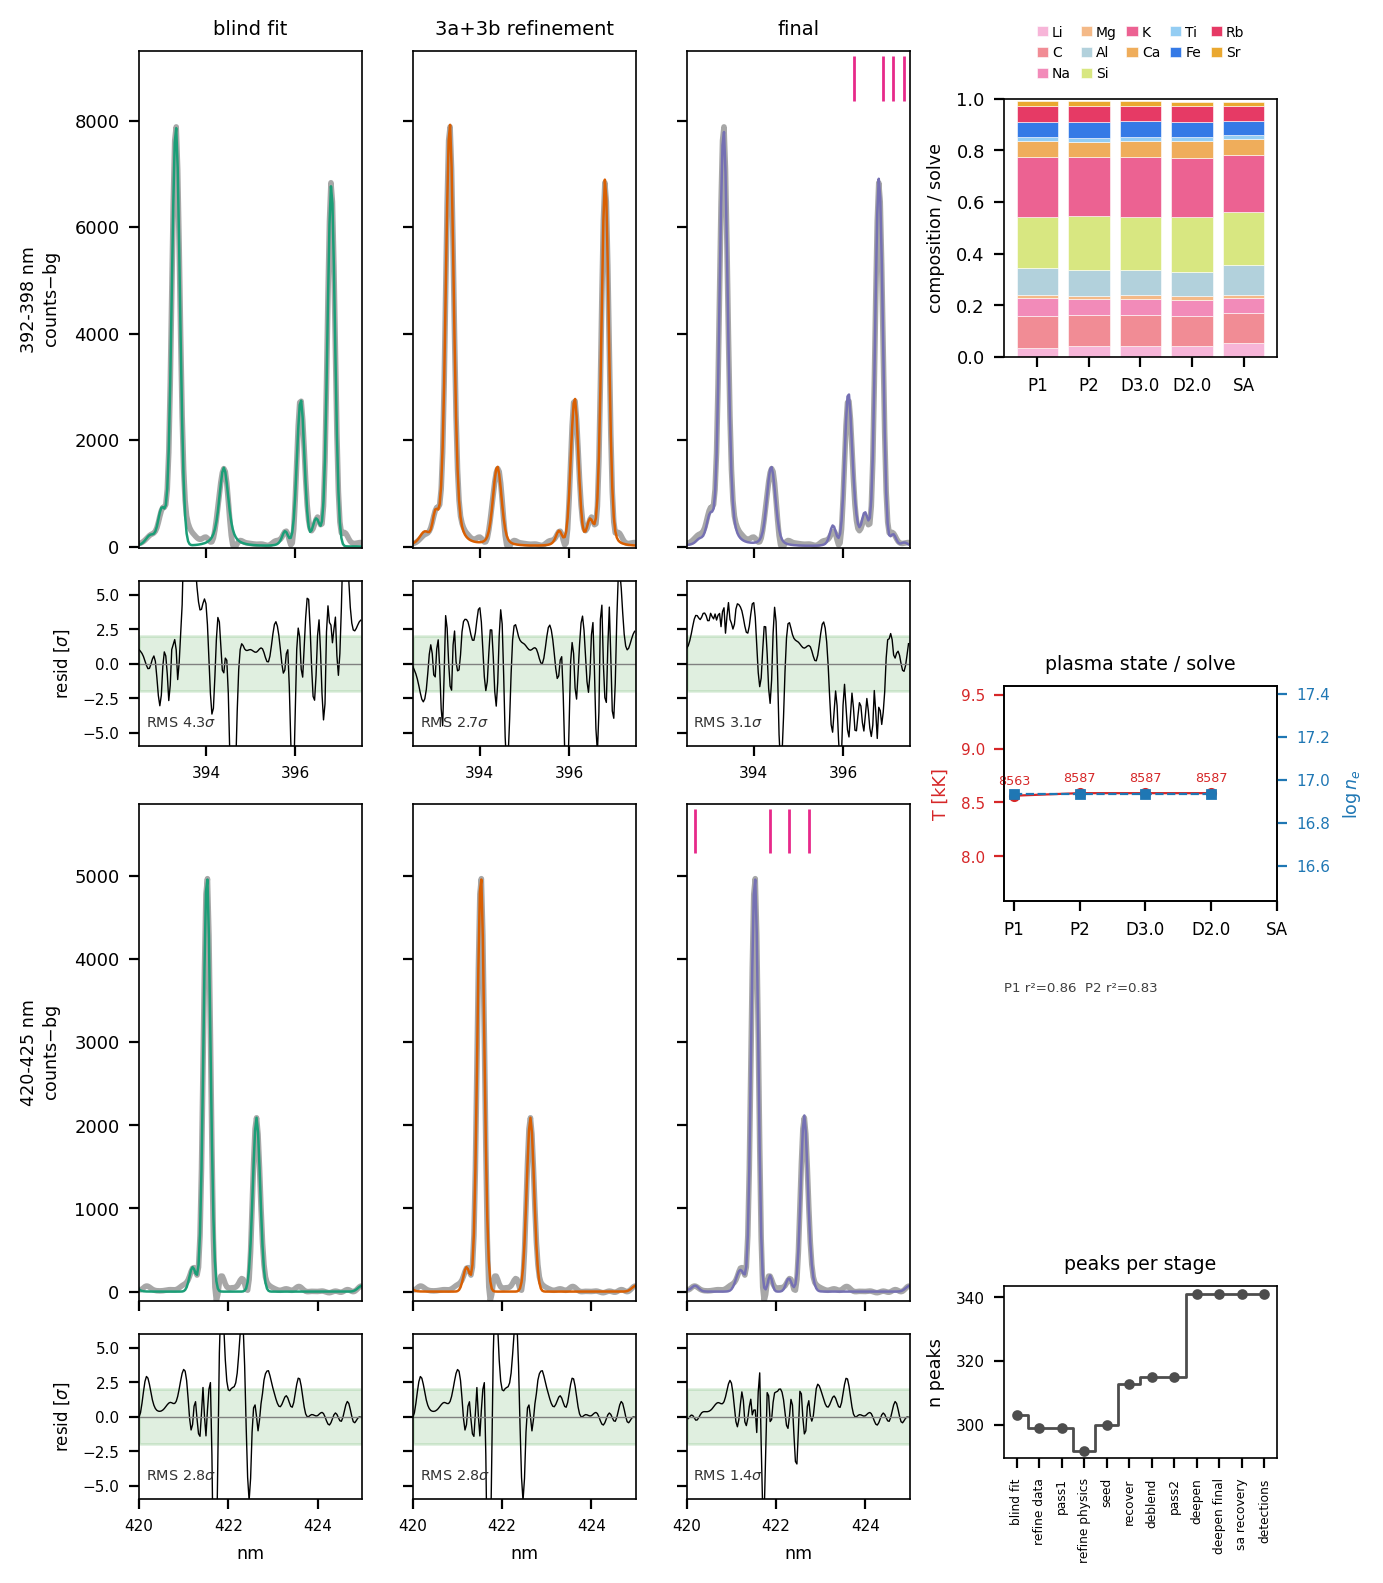
\includegraphics[width=\textwidth]{F2-walkthrough}
\caption{Stage-by-stage walkthrough of MW2-112 spectrum~1000. Left: two windows chosen for visible stage change (a Ca-rich window at \SIrange{392.5}{397.5}{\nano\metre} and a line-dense window at \SIrange{420}{425}{\nano\metre}), each shown after the blind fit, after data and physics refinement (3a+3b), and at the final model; the thick grey trace is the data, the coloured line the stage model, pink ticks mark peaks new to that column, and each residual strip (local-$\sigma$ units) carries its per-column RMS. Right: composition of every element with final fraction $\ge0.01$ across the pass-1, pass-2, accepted deepening, and self-absorption-recovery solves, the plasma state (T annotated, $r^2$ per solve), and the peak count per stage.
The peak count grows from 303 (blind) to 341 (final); the temperature moves only from \SI{8563}{\kelvin} (pass~1) to \SI{8587}{\kelvin} (pass~2) at fixed $\log_{10}(n_e/\mathrm{cm^{-3}})=16.94$, and the largest change of any element fraction across the five solves is 0.019 (Al), so the composition is stable once established; the final solve is led by K~0.22, Si~0.20, Al~0.12, and C~0.11 at $r^2=0.62$. % src: manuscript/figures/cache/mw2_1000.json
\label{fig:walkthrough}}
\end{figure*}

\subsection{Outputs}
\label{sec:wf-outputs}

The command-line entry point runs the chain over a directory of spectra in parallel workers and writes four products.
\texttt{summary.csv} has one row per spectrum: plasma parameters, detected-element fractions with statistical uncertainties, and diagnostic flags (goodness of fit, electron density at the search bound, stage disagreement, confounded and dominant-weak-shape elements, collapse rejection).
\texttt{detections.csv} is in long format, one row per sample and element: status, line support, $z$-scores, upper limits, clear-line and contested-share accounting, and the as-fit and resolved fractions.
\texttt{background\_gases.json} and \texttt{wavelength\_calibration.json} record the Ar~I and O~I evidence and the independent wavelength references, with the regions in which any correction was applied.
An inspection notebook (\texttt{fit\_inspection.ipynb}) shows the fits, refinement decisions, seeded lines and composition for one spectrum.
Unless disabled, a run manifest records the git state, configuration snapshot and input hashes, so that a reported number can be traced to the code and configuration that produced it.
The partition-function cache reduced the run time for a median spectrum of 410 peaks from
\SI{225}{s} to \SI{106}{s}. % src: git e715ff0 (MW2-112 id1518, 2.1x end to end)
